\documentclass[draftclsnofoot, onecolumn, compsoc, 10pt]{IEEEtran}

\title{\Huge Preliminary Design Document\\\large HP: Big Data Analytics\\Group 13}

\author{Oregon State University\\CS 461\\2016-2017\\\\Prepared By:\\Nic Desilets, James Stallkamp,\\and Nathaniel Whitlock}

\usepackage{titling}

\usepackage{dblfloatfix}

%\usepackage{hyperref}

\usepackage[margin=0.75in]{geometry}

\usepackage{graphicx}

\linespread{1.0} % 1.0 = single, 1.3 = 1.5, 1.6 = double

\parindent=0.0in

\parskip=0.2in

\begin{document}
\begin{titlingpage}
    \maketitle 
    
    \vspace{1in}
    \begin{abstract}
		\noindent This document is focuses on a detailed break down of "how" the individual components of our project will be implemented.
        Each of the three essential pieces: SQL development environment; parallelization and partitioning; and reporting tools are covered with fine granularity.
        We chose to focus on the design viewpoints in terms of the IEEE Std 1016-2009 document for Software Design Descriptions.
        This document outlines the path forward in terms of the viewpoints which were deemed suitable to our project.      
    \end{abstract}
\end{titlingpage}

%\tableofcontents
{\small\tableofcontents} % Reduce the size of TOC to make it 1 page
\addtocontents{toc}{\protect\thispagestyle{empty}} % Removes page number from TOC
\pagebreak

\section{Introduction}
The following sections delve into the development design and considerations that need to be outlined prior to the development cycle.
James Stallkamp covered the first four sections focusing on context, composition, logical, and dependencies viewpoints.
This was followed by three sections from Nic Desilets which covered the information, interface, and structure viewpoints.
Finally, Nathaniel Whitlock spent time on the interaction and resources viewpoints.\

\section{Glossary}
\subsection{Definitions, Acronyms, Abbreviations}

\bgroup
\def\arraystretch{1.5}
\resizebox{\textwidth}{!}{  
\begin{tabular}{| l | l |} % centered columns (4 columns)
\hline
\bf{Term} & \bf{Definition}\\ [0.5ex] 
\hline
Central Processing Unit (CPU) & The physical processor(s) in the machine that executes instructions. \\ [0.5ex]
\hline
Database & Software which stores information in an organized, easy to access manner \\ [0.5ex]
\hline
Database Administrator (DBA) & Ensures availability, reliability, performance, security, and scalability of database systems \\ [0.5ex]
\hline
HP Inc. (HP) & An American multinational information technology company headquartered in Palo Alto, California \\ [0.5ex]
\hline
Script & Refers to a collection of SQL queries in the context of this document and project. \\ [0.5ex]
\hline
SQL Developer & An integrated development environment specifically designed for both SQL queries and Oracle Database 12c. \\ [0.5ex]
\hline
Structured Query Language (SQL) & A programming language specifically designed for relational database interaction. \\ [0.5ex]
\hline
\end{tabular}
}
\egroup


%% JAMES SECTION (1-4)
\section{Context Viewpoint}
\subsection{Design Concern}
This toolkit will be used in the context of database queries that are not utilizing the host machine's resources.
The optimizer analyzes the structure of a query and allocates resources for and executes the query.
Some queries are structured such that the optimizer allocates resources in a way that much of the host machine's resources are not being utilized.
The toolkits design would help the user understand the performance of these queries that result in the under utilization of resources.
This toolkit will be a package of scripts that can be run in an environment like SQL developer.
The primary concern of the toolkit will be to gather and display performance statistics that are stored on internal performance tables within the database.
This toolkit will provide a library of scripts that can be used to gather various kinds of information on a query and how the database executed the query.
Users will be able to execute these scripts and have the output piped into files or displayed on a web page.
A User could then use this information to better understand how the database is executing a query.

\subsection{Design Elements}
This toolkit will largely be standalone, it will interact with one other entity and have one type of user.
The only other entity that this toolkit will interact with is the database that it is working with.
The SQL scripts will interact with the database by querying internal performance tables for data.
The user of this toolkit is a database user that is trying to improve or understand the performance of a query.
Users can interact by executing a script or batch of scripts and receive an output.
This output will be dependent on the user's input and scripts selected, it will be composed of various performance metrics and information about given query. 
This data can be viewed by the user in a file or through a web browser. 

\section{Composition Viewpoint}
\subsection{Design Concerns}
This toolkit will gather and display performance statistics and will do this through SQL scripts.
The purpose of the SQL scripts will be to both run a performance monitoring loop to gather runtime statistics, as well as execute test queries.
The combination of all the scripts will function as the toolkit and retrieve data on a specific query.
Each of These scripts will retrieve various pieces of data or performance metrics.
The data  will be used together to display all the required information on the performance of a specific query.

\subsection{Design Elements}
The individual scripts will be the elements of the system and will act like functions.
Each script will provide a different function by producing or retrieving a different performance statistic.
Most of the scripts or elements will be stand alone, a database user could run one or any number of the various scripts in SQL developer and receive the combined output.
The primary attribute of a script is its purpose, each script will have a different purpose, either to retrieve or output a specific performance metric.

\subsection{Function Attribute}
All of the scripts will be accessing various internal performance metric tables on the database. Each script would retrieve and analyze one of various performance metrics like memory usage, CPU usage, I/O, and many other performance metrics.
The scripts will be different in that each script will retrieve or output a different kind of statistic.
Each script within the toolkit will be providing a different a different data point on attributes like memory usage, CPU usage, etc.

\section{Dependency Viewpoint}
\subsection{Design Concerns}
This toolkit has two significant dependencies, it is however a very versatile tool because almost anyone with access to the database can use it.
Any user of the database can use this tool to retrieve information on how their query ran.
The toolkit is based on Oracle's Linux SQL technology and as a result the toolkit will only work on a Oracle SQL technology based database.
The toolkit requires Oracle SQL because the toolkit uses SQL statements to access data stored on internal performance tables.
The SQL statements also refer to entries in internal tables that may be specific to Oracle version 12c, meaning it is strongly recommended to be using this toolkit on a database that has Oracle version 12c or newer. 

\subsection{Design Elements}
The scripts in the tool kit require access to the internal performance tables on the database. 
The user must have access to those database tables for the toolkit to access them. 

%% END JAMES

%% NIC'S SECTION (5-8)
\section{Information Viewpoint}
\subsection{Design Concerns}
The primary persistent data structure and source of data for the toolkit will be the internally managed performance metrics tables contained in Oracle Database 12c.
Users will be able to request information about a particular query ran against the database through the use of this toolkit and these internal performance tables.
The data returned from the toolkit regarding a particular query can include information such as time elapsed, processor usage, memory consumption, degrees of parallelism, and other related metrics.

\subsection{Design Elements}
The data items that are retrieved by the toolkit are stored in a permanent data store (Oracle 12c).
Access of this data is provided through the use of SQL Developer in which the toolkit scripts are intended to be run with.
SQL Developer initiates a connection to the database to retrieve the relevant performance information needed by the toolkit scripts. 

More specifically, the information that is retrieved by the toolkit comes from different tables within the database.
The records stored in these database tables are generated after the user executes a query.
After completion of a query, the toolkit can then be used to query the database again for metrics information about the previous query ran by the user.
This information is then processed and returned to the user in a human readable format.

\subsubsection{Data Attribute}
The metrics information that the database contains spans a broad range of different types of information used for profiling the performance of queries.
The specific types of this information ranges from numbers, strings, to date representations.
For example, timing information is represented as numbers, metrics descriptions are represented as strings, and start and end times would be date representations.

All of this information is categorized and put into specific tables that relate to a certain domain of information relating to a query.
Examples of this can include storing memory usage information into a table that describes how much memory was consumed over time when processing a particular query.
The data stored in these tables is intended to be used to offer insights into query performance.

\section{Interface Viewpoint}
\subsection{Design Concerns}
The primary interface for this toolkit is going to be SQL Developer. 
The toolkit itself consists of SQL queries that are to be executed inside the SQL Developer environment.
Users will select which toolkit query they want to run based on what type of information they need. Upon selecting a query, the user will then load it into SQL Developer which sends the query to the database.
Results returned by the database will then be presented to the user in a human readable format.

\subsection{Design Elements}
The primary elements of SQL Developer include the SQL Worksheet window.
This where queries will be loaded and then sent off to the database for execution.
Once the database has completed processing a particular query, the results from the database are then returned and presented to the user. 
These results are contained in a new window within the SQL Worksheet window.
Users will be able to scroll through the results if there is a large amount of information.

\subsection{Examples}
\begin{center}
	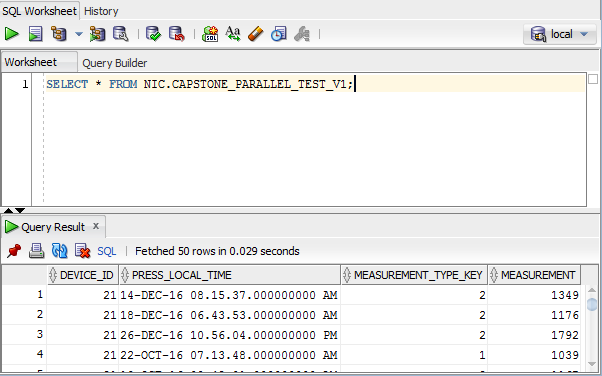
\includegraphics[width=5in]{sql_worksheet_example.png}

	Fig 1. An example SQL query in the SQL Worksheet window. Query results are shown in the Query Results window.
\end{center}

\subsection{Example Languages}

\section{Structure Viewpoint}
\subsection{Design Concerns}
The two primary structures involved with the toolkit are SQL Developer and Oracle Database 12c.
Oracle Database 12c is a permanent data store and SQL Developer is an environment that is used to interface and interact with Oracle Database.
SQL Developer must first initiate a connection to Oracle Database 12c in order to execute any queries.
If the connection is successful, the user can then start loading and executing queries via SQL Developer's database connection.

\subsection{Design Elements}
SQL Developer connects to Oracle Database 12c in order to retrieve information contained in its data store.
The purpose of SQL Developer is to serve as a work space for the user to input queries, have the queries executed, and view the output returned by the queries.
The database on the other hand is a data store that houses information relating to HP PageWide Press printers and also internal metrics relating to query performance.
The connection from SQL Developer to Oracle Database 12c serves as the means of bi-directional communication between the two structures.

%% END NIC

%% NATE'S SECTION (9-12)
\section{Interaction Viewpoint}

\subsection{Design Concerns}
The main design concern in terms of the interaction between system entities is an open line of communication with the Oracle database.
If this connections is severed, then there is no way for the user's personal computer to execute a query on the database.
Therefore, the toolkit will not perform and the transaction will be impossible. 
In terms of allocation of responsibilities in collaborations with the toolkits use at HP, the user's machine will only be responsible for composing the query and sending it through to the database running on the server.
The calculations and each procedural step of the toolkit analysis will be processed remotely and the results and statistical report should return to the user.

\subsection{Design Elements}
The entities involved at various levels of action are as follows; Engineer/DBA, personal computer, server, and Oracle database.
During the transaction from the user to the server there are multiple wait instances where one of the host systems sits idle waiting for the final result response.
Methods used in the communication process are beyond the scope of our toolkit and will be handled by higher order systems.

\subsection{Examples}
The process of interaction between the entities involved in a transaction with our toolkit can be summarized as request from a user and a response from the target Oracle database. In this example the response is composed of the users desired results and a performance statistic report.
The report will have information about hardware optimization and run-time analysis.
This information can then be used to quantitatively compare queries run with different system parameter settings, by comparing the run-time of multiple experiments a optimal design can be identified. 

% Figure here
\begin{center}
	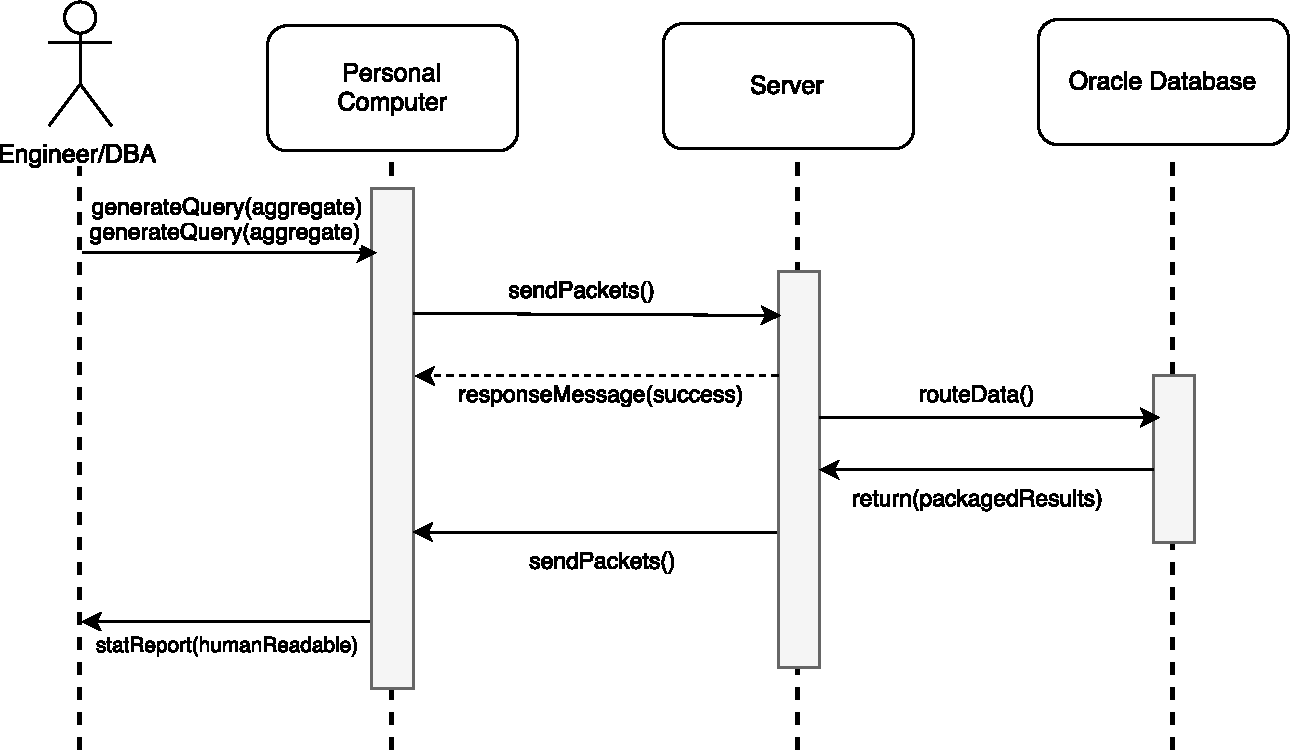
\includegraphics[width=6in]{Sequence_Diagram.pdf}

	Fig 2. Sequence of actions once query of interest and toolkit are executed by the user.
\end{center}


\section{Resource Viewpoint}
\subsection{Design Concerns}
The purpose of the toolkit is to monitor the system processing a query in order to generate a report which outlines the performance metrics.
There should be concern placed on the overhead processing time of the toolkit query.
The only inherent performance concerns for our toolkit would be the syntax used to build the toolkit query, which could be evaluated with the SQL explain plan. This toolkit should be portable to all systems capable of hosting Oracle database software so it should be lightweight in terms of size. 

\subsection{Design Elements}
The design entities we have considered are modeled after the system properties we are interested in measuring.
Time elapsed is the main entity but we also have CPU cores, disk I/O, and parallel coordinator.
The time elapsed entity will allow us to track the processing time for the query being evaluated, this will be useful when comparing the run-time of identical queries given different configuration.
The CPU cores entity will provide information about how many individual cores were used out of the total available cores and how much work each was assigned.
The disk I/o entity will be used to monitor swap space needed due to lack of physical memory resources.
Together CPU cores and disk I/O will help us monitor how much of the available hardware is being utilized during SQL processing.
Finally, the parallel coordinator entity will provide information about the type and level of parallelism that was used.

In terms of constraints for each entity, the time elapsed entity should ideally be as low as possible to enable near real time access to WebPress performance data.
There are a total of 72 core processors available during query execution, so the CPU core entity is limited by that number.
The disk I/o entity should ideally have a minimal amount of activity meaning that the SQL plan the optimizer put together was efficient and the initial data fetch was as well.
If a query is executed with parallelism enabled and a hint for a specific number ($n$) of individual processors, then each one of the available cores should be used.

\subsection{Examples}
By isolating each one of the above stated entities we will be able to generate a report with enough information to tune a users queries as well as provide the metrics needed for quantitative comparison.
An example of this would be testing the effectiveness of a table partition design in respect to a query that performed calculations on specific values and took a large amount of time.
By monitoring these entities, we will be able to see how many cores were made available to the coordinator, how much swap space was used, and how many parallel processes were estimated to be efficient.
Additionally, we will have a custom metric calculated from time elapsed from the point of query execution.

% Figure here
\begin{center}
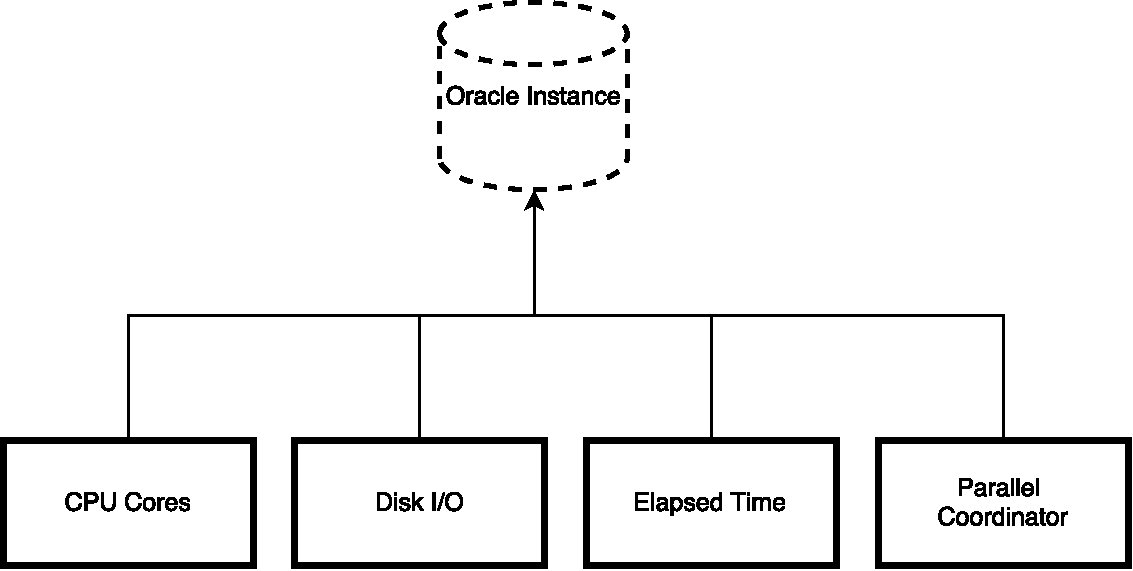
\includegraphics[width=5in]{Class_Diagram.pdf}

	Fig 3. Simple visualization of the resource entities and the database.
\end{center}
%% END NATE

\section{Conclusion}
The toolkit that we are creating consists of multiple interacting entities including the end users, Oracle Database 12c, and SQL Developer. 
During the technology review phase we carefully reviewed our options for these entities and chose technologies that were best suited for this project. 
This document embodies a solution to bring all of these technologies and entities together in order to assist database administrators with evaluating query performance. 


\vspace{4in}

\noindent\begin{tabular}{ll}
\makebox[2.5in]{\hrulefill} & \makebox[2.5in]{\hrulefill}\\
Kirby Sand & Date\\[8ex]% adds space between the two sets of signatures
\makebox[2.5in]{\hrulefill} & \makebox[2.5in]{\hrulefill}\\
Andy Weiss & Date\\[8ex]%
\makebox[2.5in]{\hrulefill} & \makebox[2.5in]{\hrulefill}\\
Nic Desilets & Date\\[8ex]%
\makebox[2.5in]{\hrulefill} & \makebox[2.5in]{\hrulefill}\\
James Stallkamp & Date\\[8ex]%
\makebox[2.5in]{\hrulefill} & \makebox[2.5in]{\hrulefill}\\
Nathaniel Whitlock & Date\\[8ex]%
\end{tabular}


\end{document}
